\section{问题二：分组优化与NIPT时点决策模型}

问题二要求为不同身体质量指数即BMI的男胎孕妇制定分组方案，并为各组确定唯一的最佳NIPT检测时点。该策略的目标是最小化全体孕妇的潜在风险总和。决策过程需要在两种风险之间权衡，一是过早检测可能因Y染色体浓度不达标而失败，二是过晚检测会缩短临床干预的有效时间。为处理此权衡问题，本文建立了一个包含孕妇分组与时点选择的双层决策模型。具体机制如\cref{fig:flowchart_q2}所示。


\begin{figure}[h!]
\centering
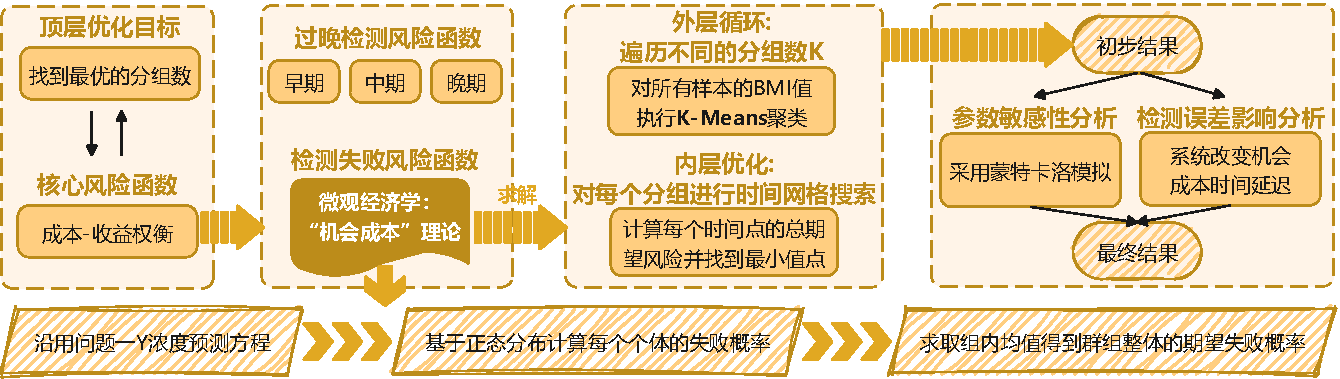
\includegraphics[width=\textwidth]{figs/4问题二/问题二.pdf}
\caption{问题二流程图}
\label{fig:flowchart_q2}
\end{figure}
\subsection{风险量化与优化目标}
模型顶层的优化目标为寻找最优的分组数量K，使所有组别按其人口比例加权的期望风险总和达到最小。总期望风险$E[R_{total}]$的数学表达式为
\begin{equation}
\min_{K, \{t_i\}} E[R_{total}] = \sum_{i=1}^{K} \frac{n_i}{N} \cdot R_i^*(t_i^*)
\end{equation}
其中$N$为孕妇总数，$n_i$为第$i$组的人数，$R_i^*(t_i^*)$是第$i$组在其最优检测时点$t_i^*$下的最小期望风险。对于任何分组$i$，其在特定检测时点$t_i$的总期望风险$R_i(t_i)$由两部分构成
\begin{equation}
\min_{t_i} R_i(t_i) = R_{late}(t_i) + R_{fail}(t_i)
\end{equation}
此处的$R_{late}(t_i)$是因推迟检测累积的健康风险，$R_{fail}(t_i)$是因检测失败造成的机会成本风险。$R_{late}(t_i)$随时间增加，而$R_{fail}(t_i)$随时间减少。两者叠加形成的$R_i(t_i)$总风险曲线上存在一个最小值点，该点对应的时间即为最优检测时点。

\subsection{风险函数的数学构建}
为量化延迟检测的健康风险，依据题目描述的早、中、晚三个孕期风险等级，构建了一个分段函数。该函数通过线性和指数部分描述风险增长先缓后急的特征
\begin{equation}
R_{late}(t_i) =
\begin{cases}
\frac{2}{14}(t_i - 70) & \text{若 } 70 \le t_i \le 84 \\
2 + \frac{4}{105}(t_i - 84) & \text{若 } 84 < t_i \le 189 \\
0.2225 \cdot e^{0.0243 \cdot t_i} & \text{若 } 189 < t_i \le 210
\end{cases}
\end{equation}
在此函数中，$R_{late}(t_i)$代表在第$t_i$天检测时，因延迟累积的健康风险值，自变量$t_i$为天数。

对于检测失败的风险，本文使用了微观经济学中的机会成本理论进行量化。选择在特定时点检测，若因Y染色体浓度不达标而失败，其后果是必须延后进行下一次检测。此延后构成一种机会成本，其代价是在等待重新检测期间，孕妇所承受的额外健康风险增量。因此，检测失败风险$R_{fail}(t_i)$被定义为失败概率与失败所致机会成本的乘积
\begin{equation}
R_{fail}(t_i) = E[P_{fail, group}(t_i)] \times W(t_i) \times \left[ R_{late}(t_i + \Delta t) - R_{late}(t_i) \right]
\end{equation}
其中，$E[P_{fail, group}(t_i)]$是该分组在时点$t_i$的期望失败概率。$W(t_i)$是随时间变化的价值权重函数。$\Delta t$代表两次检测的时间间隔，本文设定为14天。最后的差值项是对机会成本的量化，表示因本次检测失败而被迫推迟$\Delta t$天后，带来的健康风险净增量。

时间价值权重$W(t_i)$用以体现不同孕周决策价值的差异，其形式为一个反向逻辑斯谛函数
\begin{equation}
W(t_i) = 0.01728 + \frac{0.16344}{1 + e^{0.1(t_i - 154)}}
\end{equation}
此函数中变量$t_i$为检测时点的天数，函数输出值$W(t_i)$为该时点对应的决策价值权重。

\subsection{失败概率的预测模型}
为计算特定分组在特定时间的期望失败概率$E[P_{fail, group}(t_i)]$，需要一个能够预测Y染色体浓度的数学模型。该模型需能反映群体趋势与个体差异。本文采用问题一建立的非线性混合效应模型进行预测。模型形式为
\begin{equation}
\hat{Y}_{ij} = (\beta_0 + u_{0,i}) + (\beta_1 + u_{1,i})\text{GW}_{ij} + \beta_2\text{GW}_{ij}^2 + \beta_3\text{GW}_{ij}^3 + \beta_4\text{BMI}_{ij}^3
\end{equation}
其中，$\hat{Y}_{ij}$是对第$i$位孕妇在第$j$次检测时Y染色体浓度的预测值。参数$\beta_0$至$\beta_4$是固定效应系数，代表样本总体的平均变化规律。$u_{0,i}$与$u_{1,i}$是随机效应项，代表第$i$位孕妇的个体基线水平与孕周影响的个体差异。

基于此模型，可计算任一孕妇$i$在未来时间点$t$的失败概率。检测失败定义为Y染色体浓度低于百分之四的阈值。个体失败概率$P_{fail,i}(t)$的计算用到模型的预测值$\hat{Y}_i(t)$与模型残差的标准差$\hat{\sigma}_{\epsilon}$，其计算式为
\begin{equation}
P_{fail,i}(t) = P(Y_i(t) < 0.04) = \Phi\left(\frac{0.04 - \hat{Y}_i(t)}{\hat{\sigma}_{\epsilon}}\right)
\end{equation}
其中$\Phi(\cdot)$是标准正态分布的累积分布函数。一个分组的整体期望失败概率，是该分组内所有个体失败概率的算术平均值
\begin{equation}
E[P_{fail, group}(t)] = \frac{1}{n_{group}} \sum_{i \in group} P_{fail, i}(t)
\end{equation}
此处的$n_{group}$是该分组内的孕妇总人数。该计算方法将每位孕妇的个体特征都纳入考量，从而得到整个群体的风险评估。\cref{fig:q2_individual_prob}展示了混合效应模型为部分孕妇生成的Y染色体浓度达标概率预测曲线，体现了模型捕捉到的个体间差异。

\begin{figure}[h!]
\centering
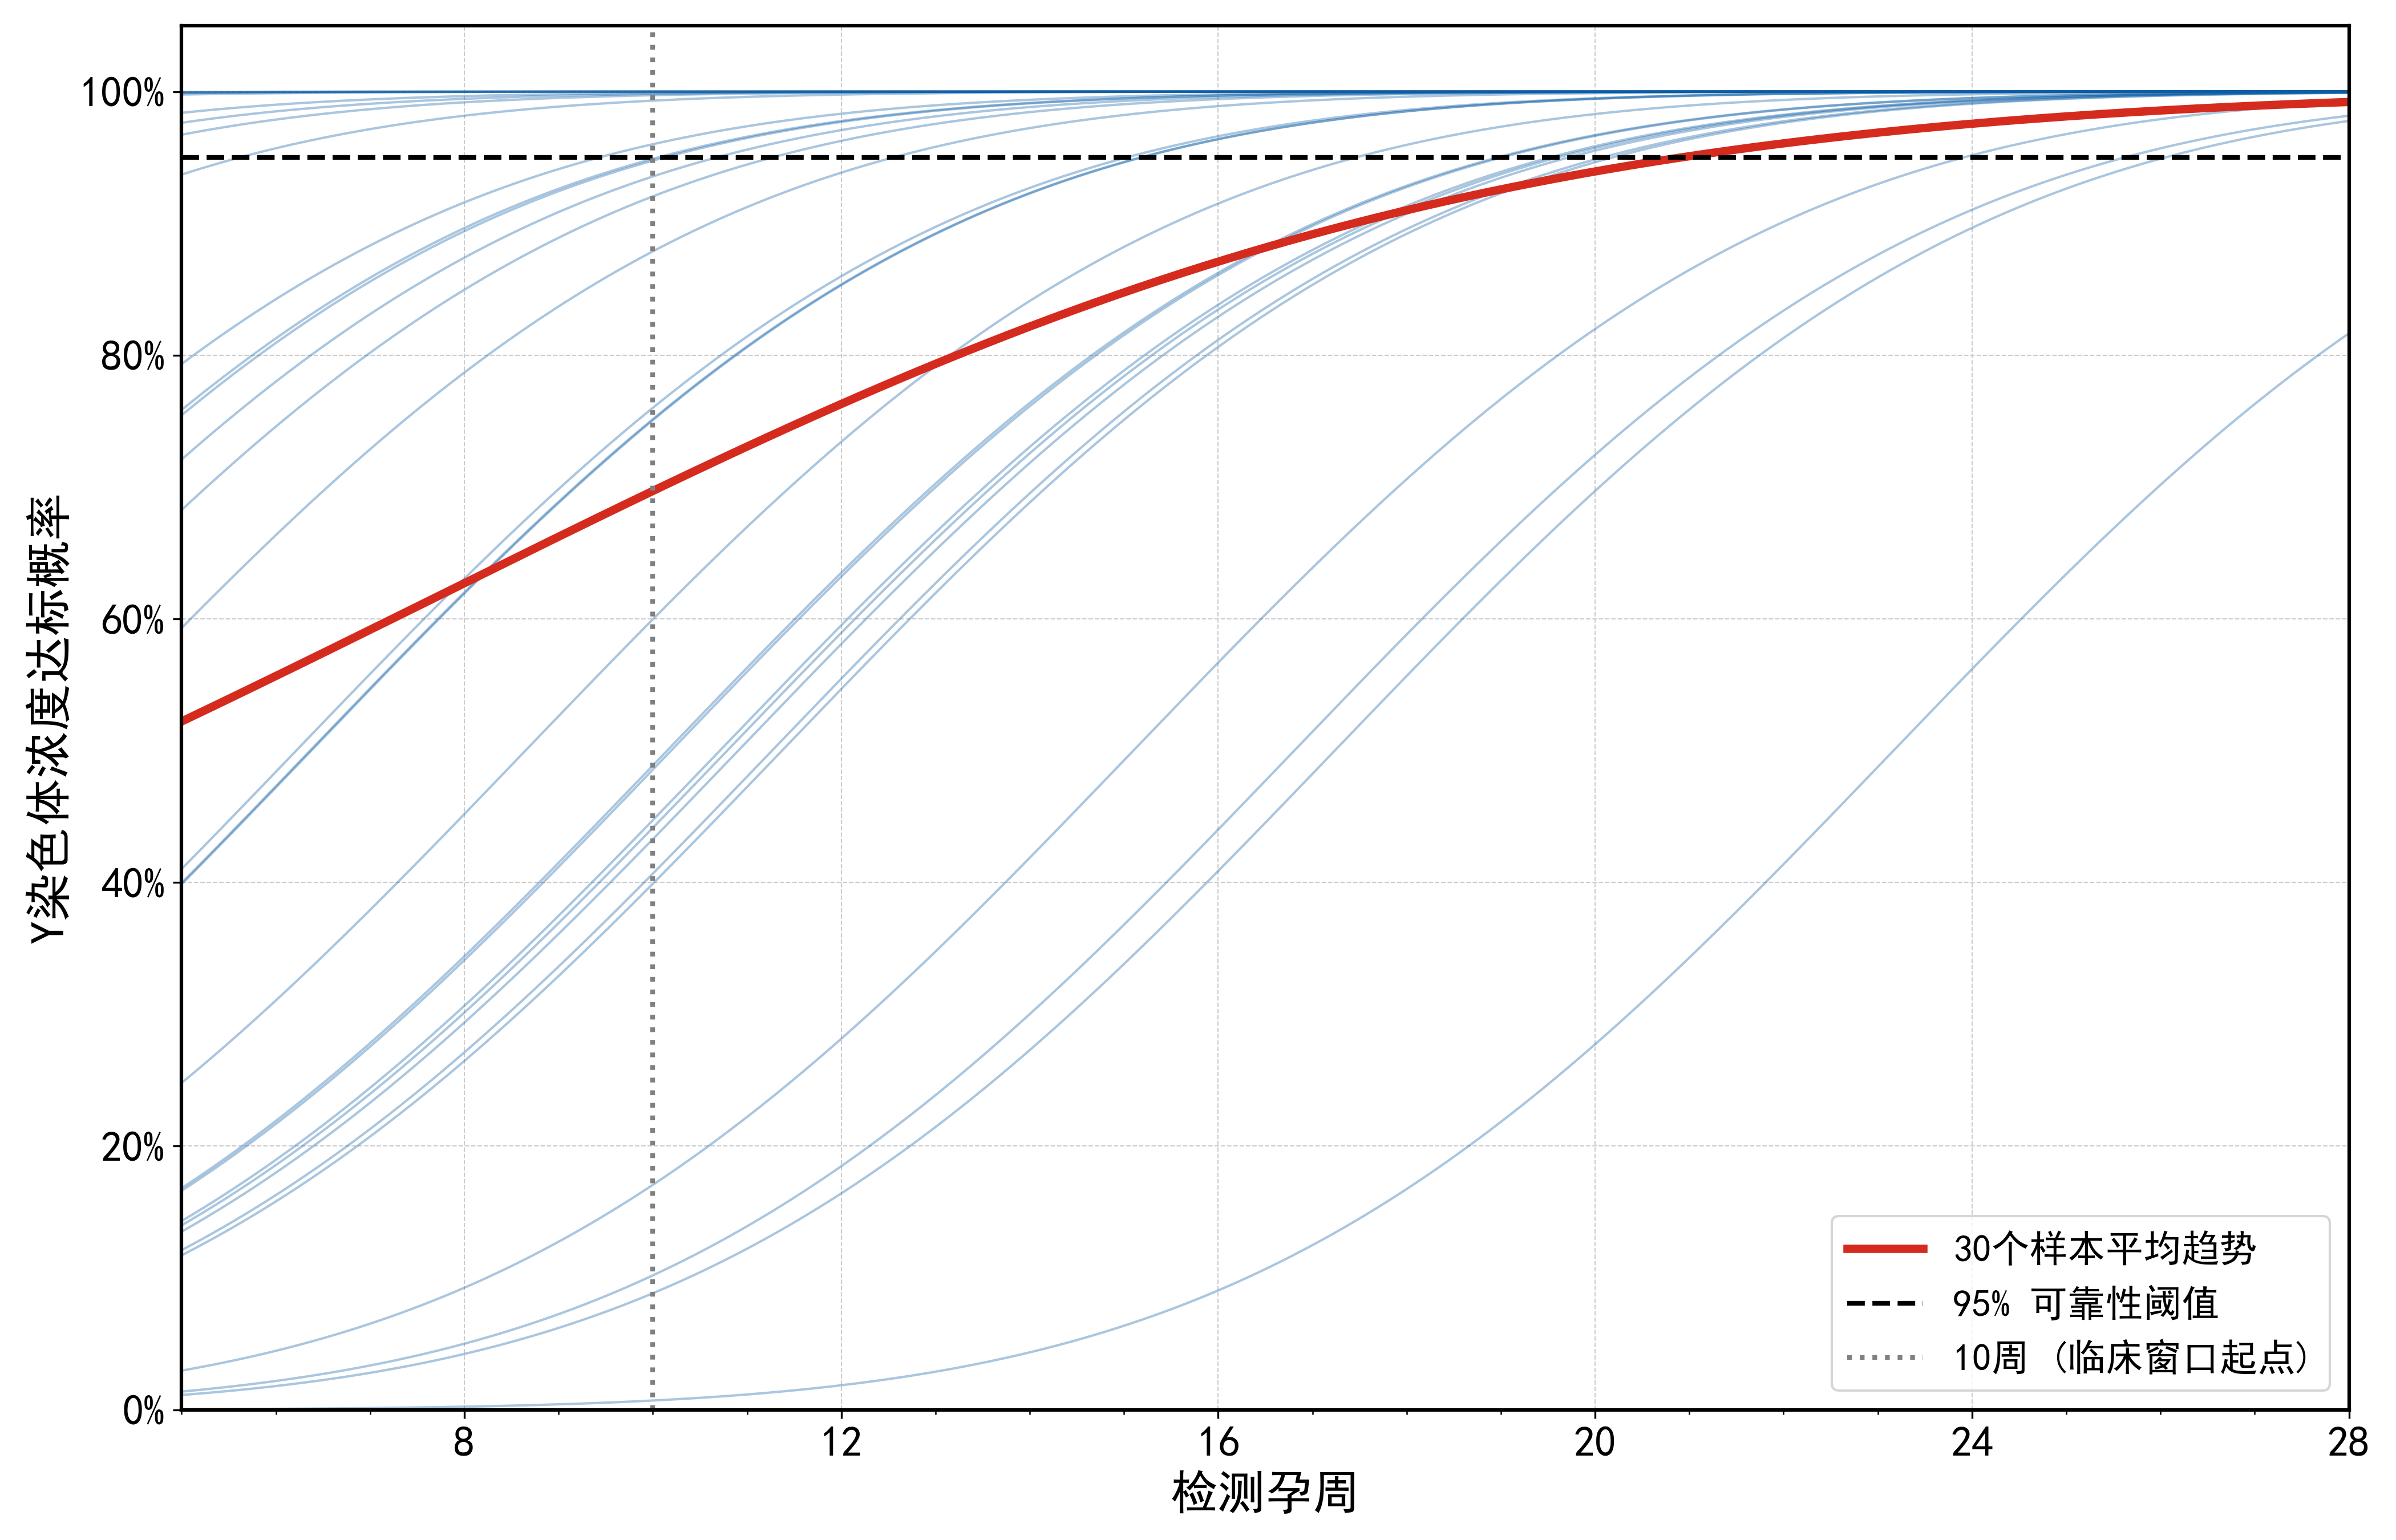
\includegraphics[width=0.8\textwidth]{figs/4问题二/图4_30个孕妇个体概率趋势.png}
\caption{混合效应模型预测的个体Y染色体浓度达标概率变化轨迹}
\label{fig:q2_individual_prob}
\end{figure}

\subsection{模型求解与最优方案确定}
模型的求解采用K均值聚类与网格搜索结合的双层优化算法。外层循环遍历分组数K从2至8。对每个K值，先对所有样本的BMI进行K均值聚类以完成分组。随后在内层优化中，对每个组别，在70天至196天的时间范围内进行网格搜索，逐日计算其总期望风险，取风险最低点对应的时间作为该组的最佳NIPT时点。最后，比较不同K值下的加权平均总风险，风险最低者对应的K值即为最优分组数。

\begin{figure}[h!]
\centering
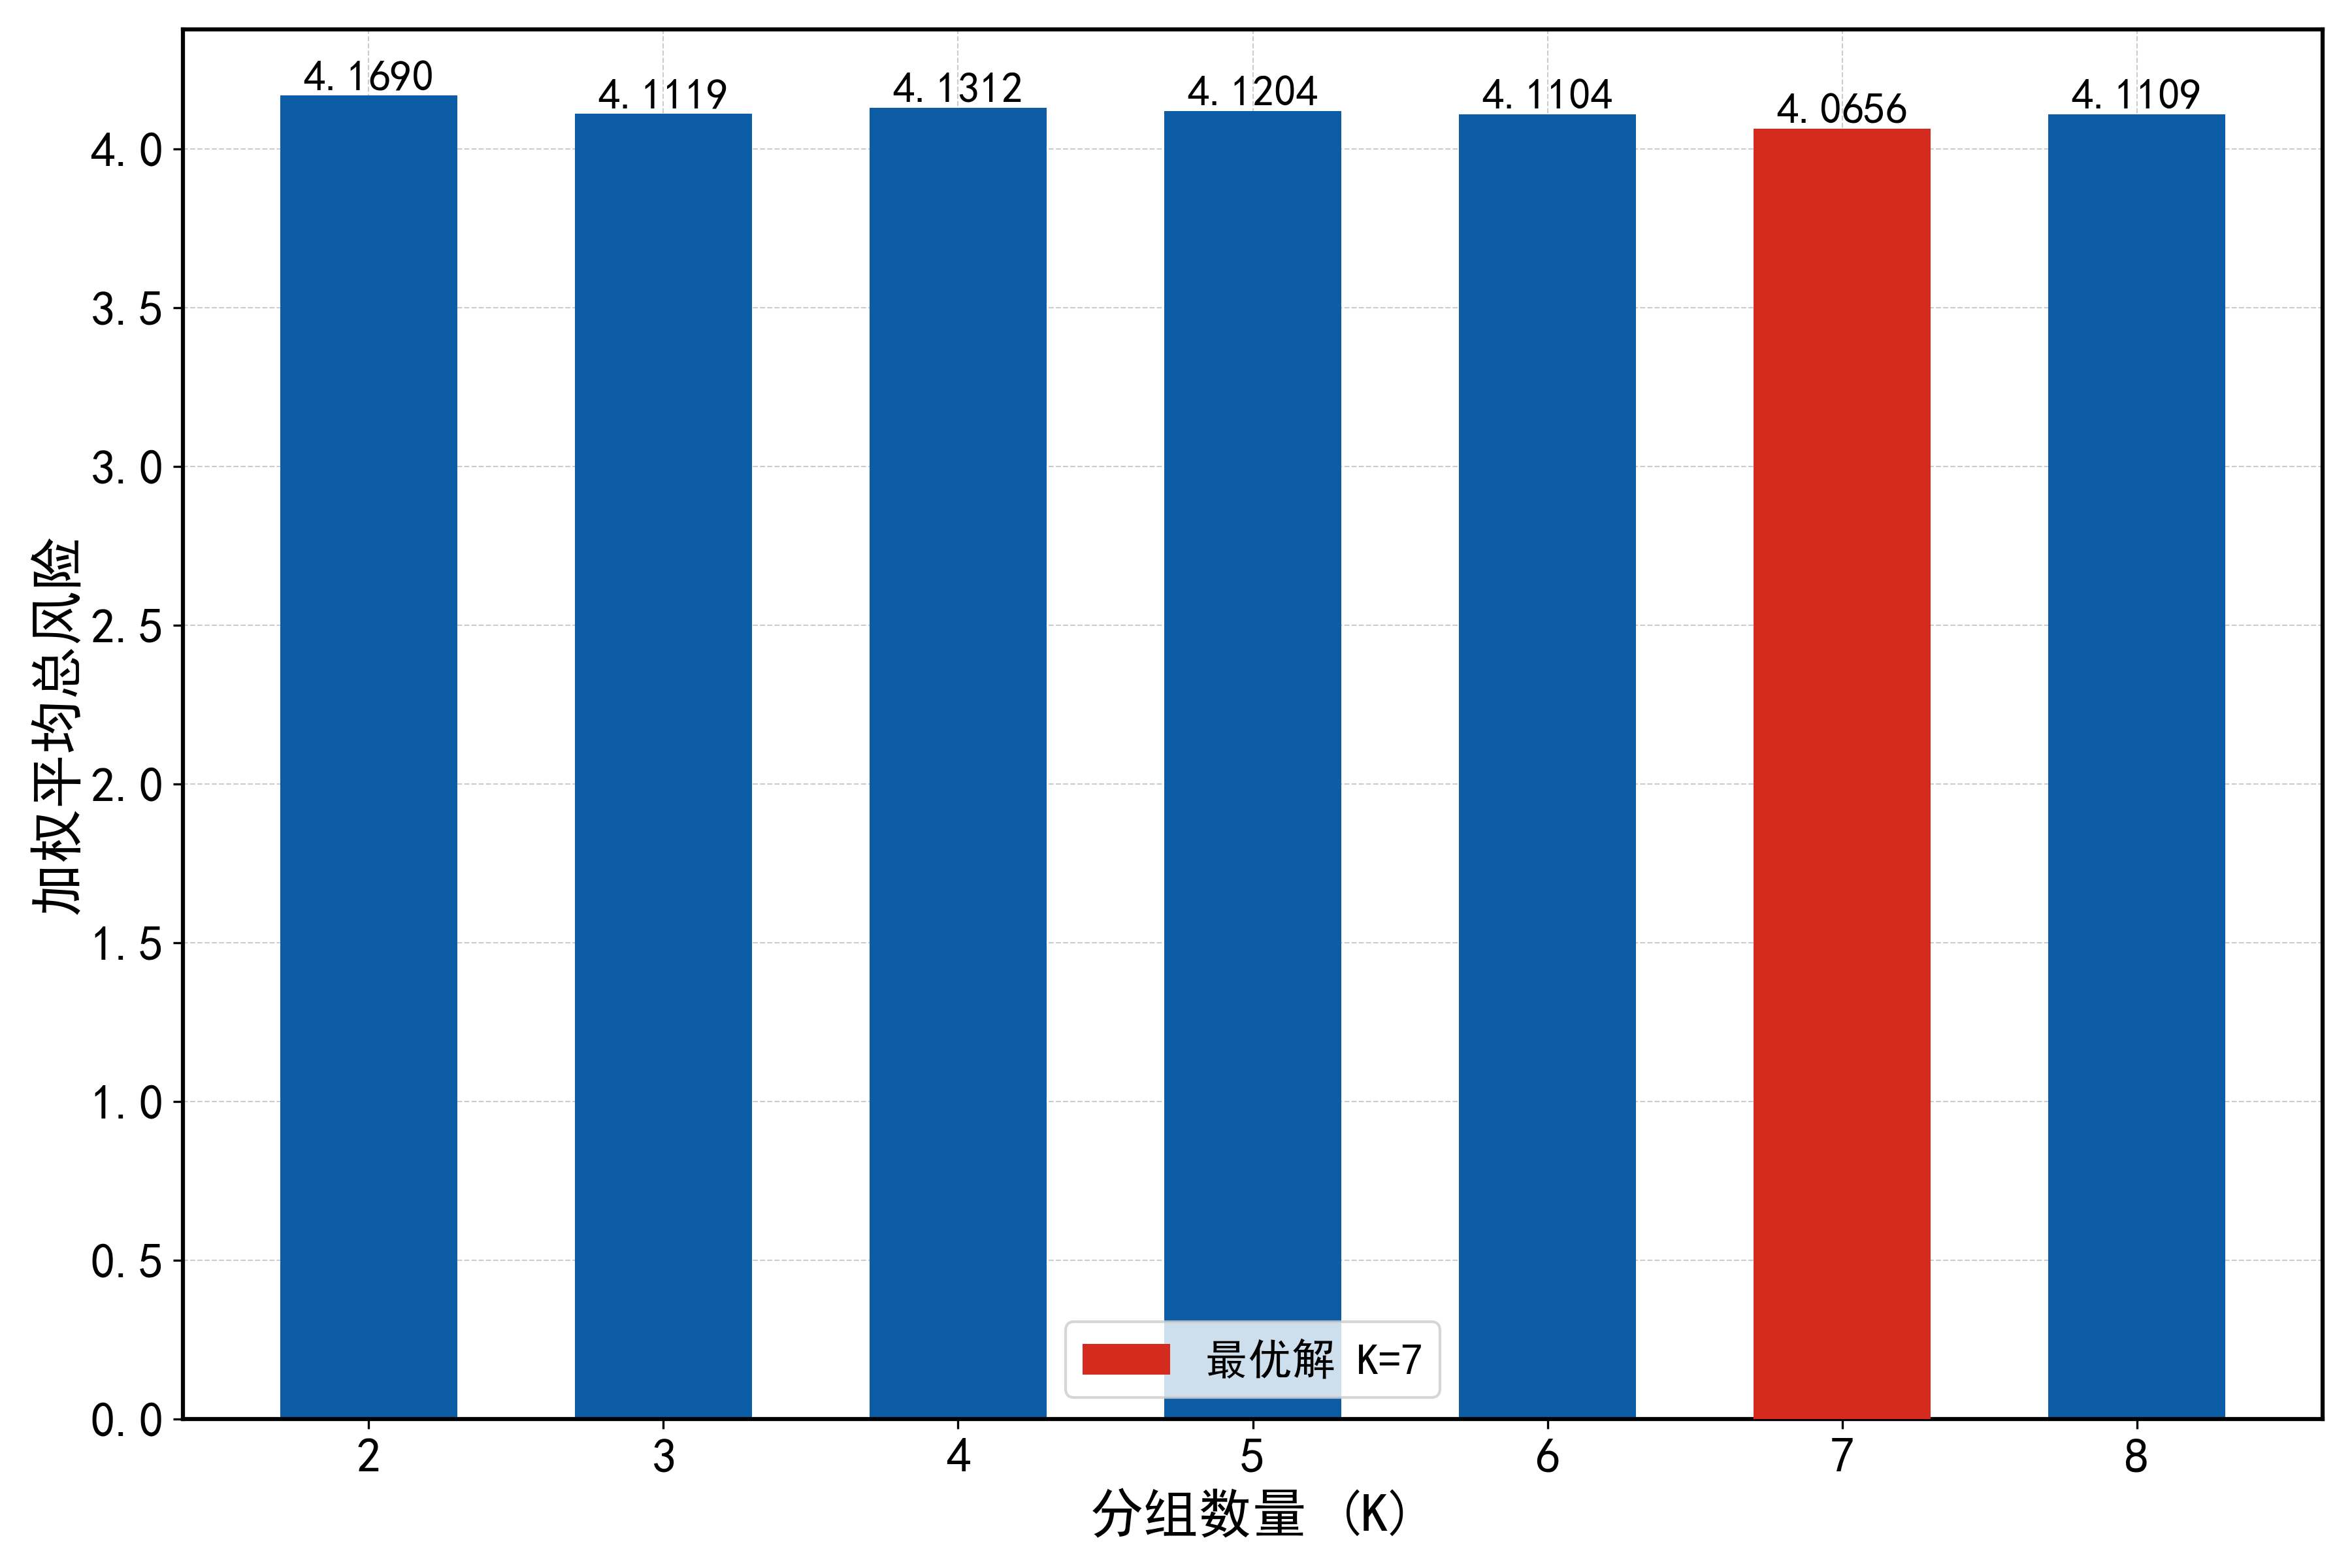
\includegraphics[width=0.8\textwidth]{figs/4问题二/图3_不同K值总风险对比.png}
\caption{不同分组数K对应的加权平均总风险}
\label{fig:q2_k_comparison}
\end{figure}

选择最优分组数的过程如\cref{fig:q2_k_comparison}所示。图中以柱状图形式展示了不同分组数K对应的加权平均总风险值。计算结果表明，当分组数K等于7时，加权平均总风险达到所有候选方案中的最小值4.0656。因此，将孕妇群体划分为七个组别是当前模型下的最优策略。

\begin{figure}[h!]
\centering
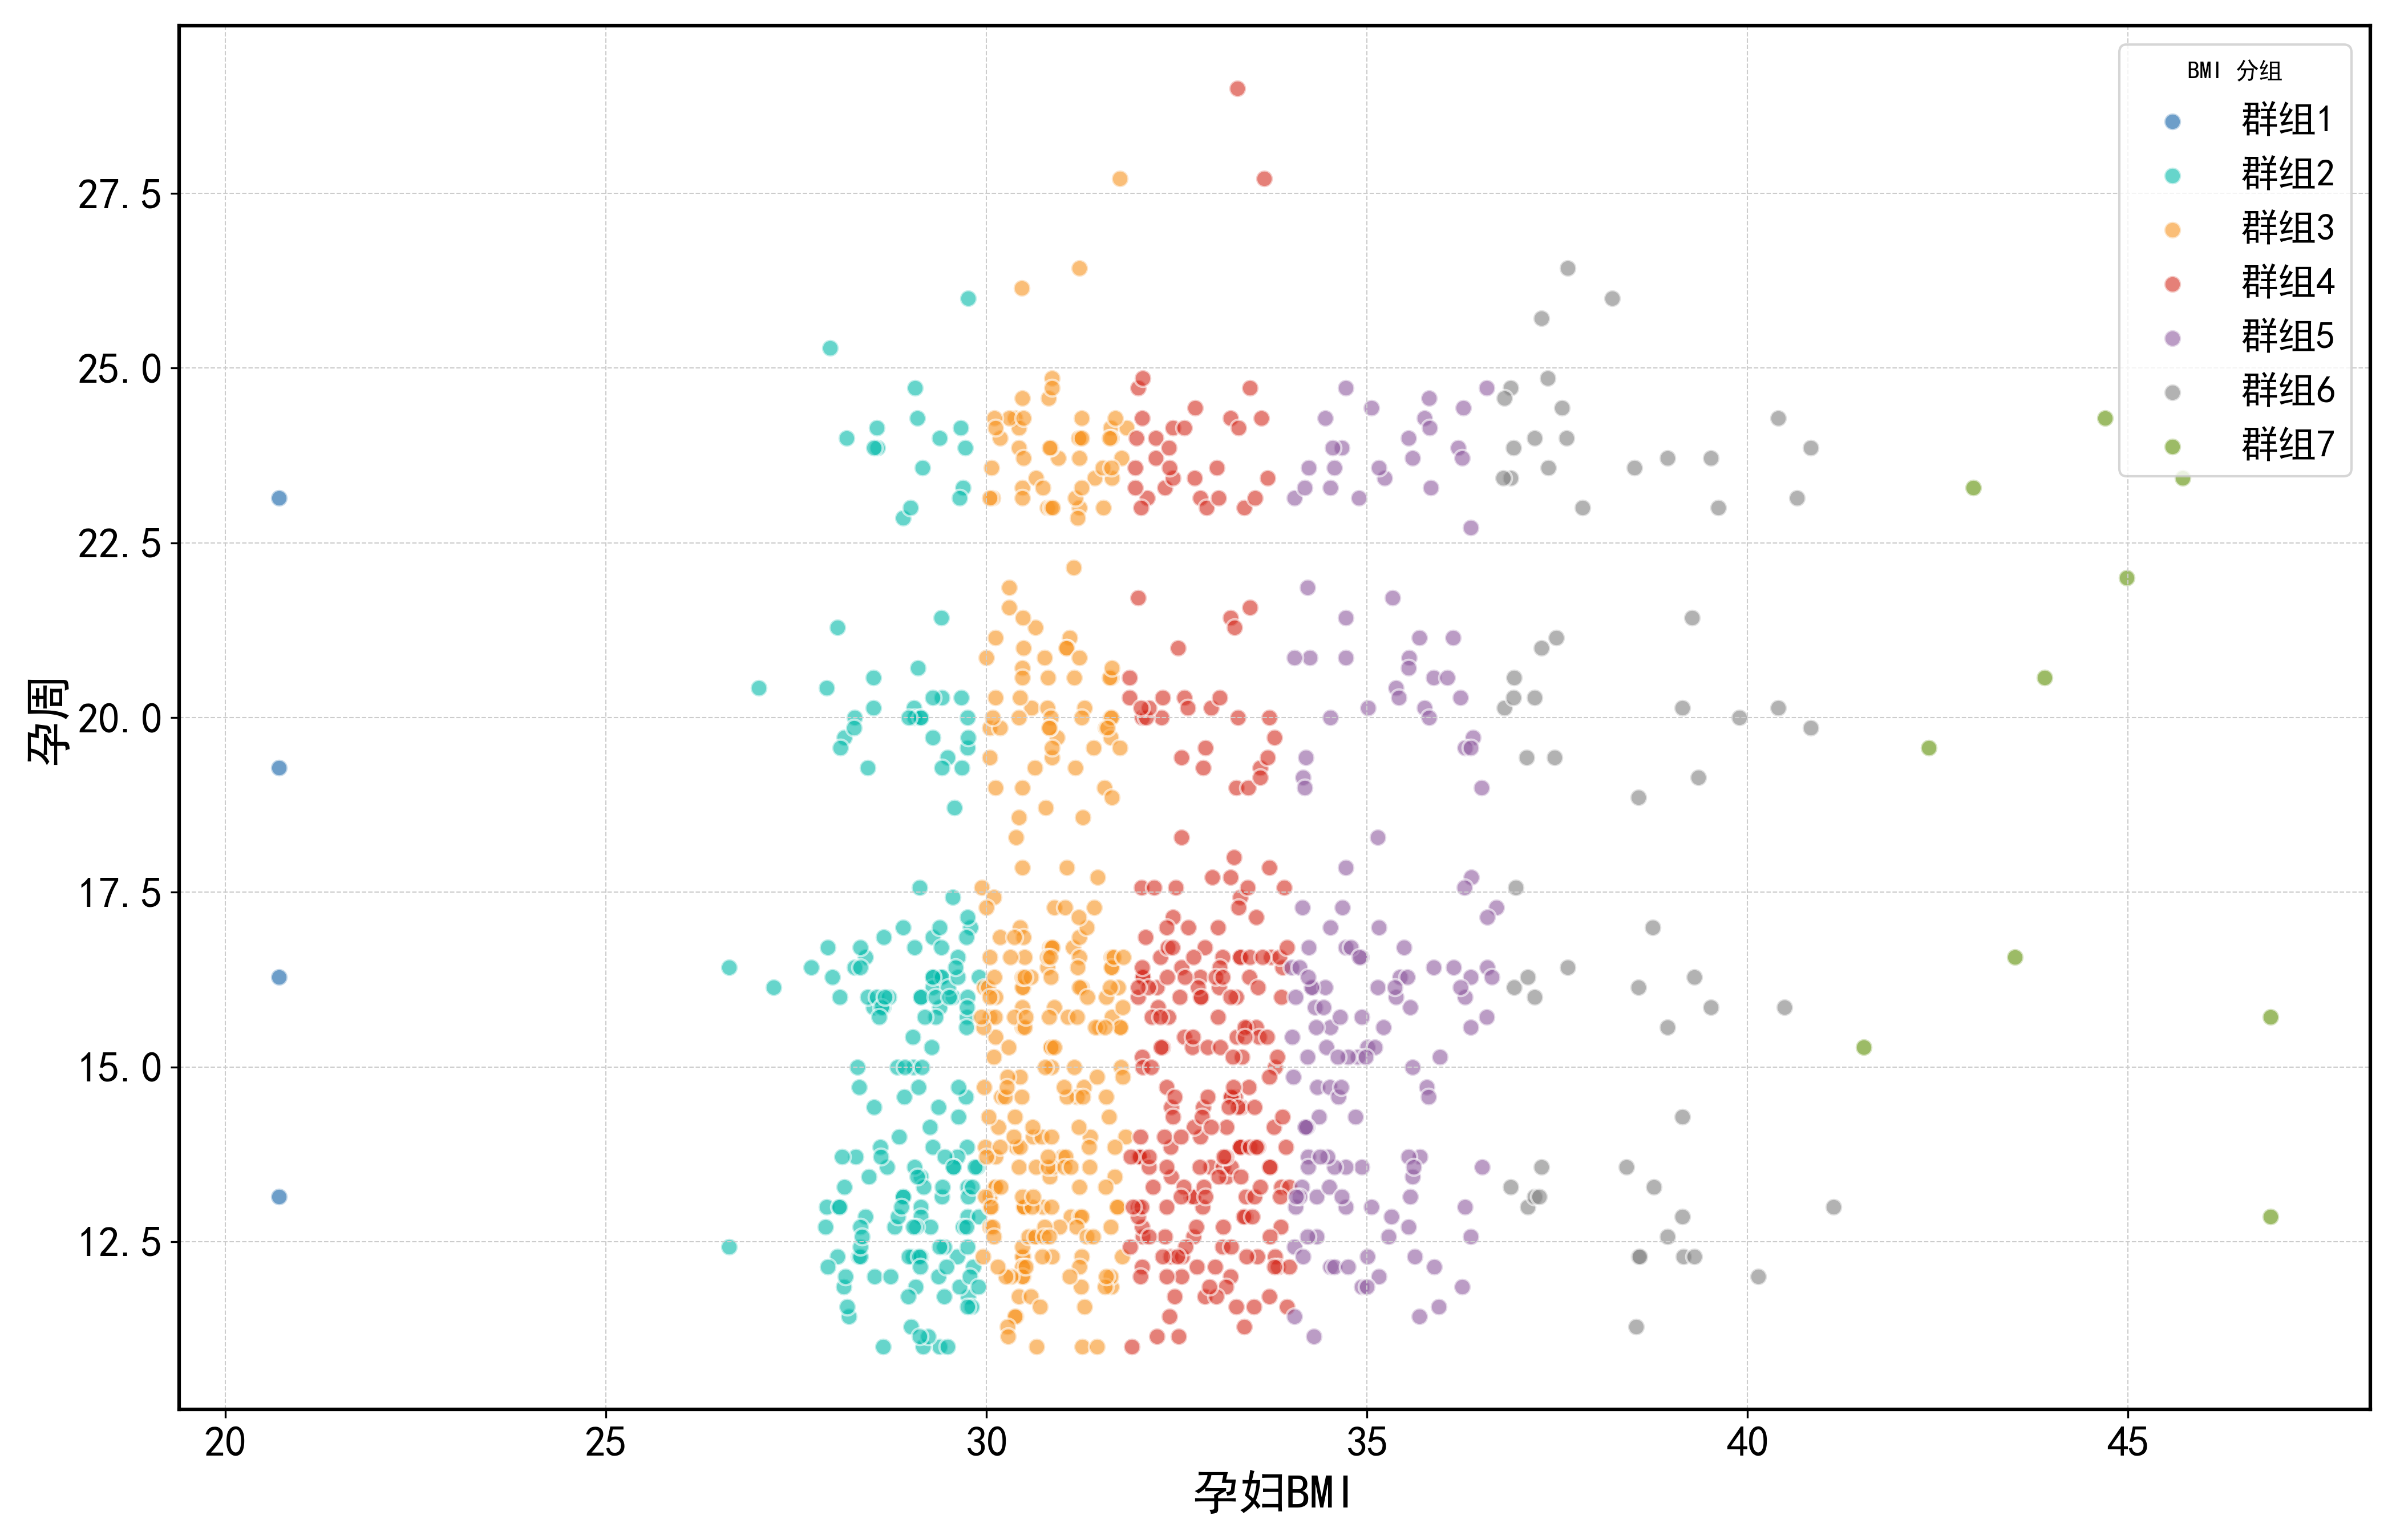
\includegraphics[width=0.8\textwidth]{figs/4问题二/图2_最优分组数K7_BMI聚类结果.png}
\caption{最优分组数K等于7时基于BMI的聚类结果}
\label{fig:q2_clusters}
\end{figure}

在确定最优分组数为7后，对孕妇BMI进行聚类的结果可见于\cref{fig:q2_clusters}。该图以散点形式展示了每一个样本，并用不同颜色标识其所属的群组。七个群组沿孕妇BMI轴向分布，形成了七个相互邻接的区间，体现了对孕妇群体的细分。

\begin{figure}[h!]
\centering
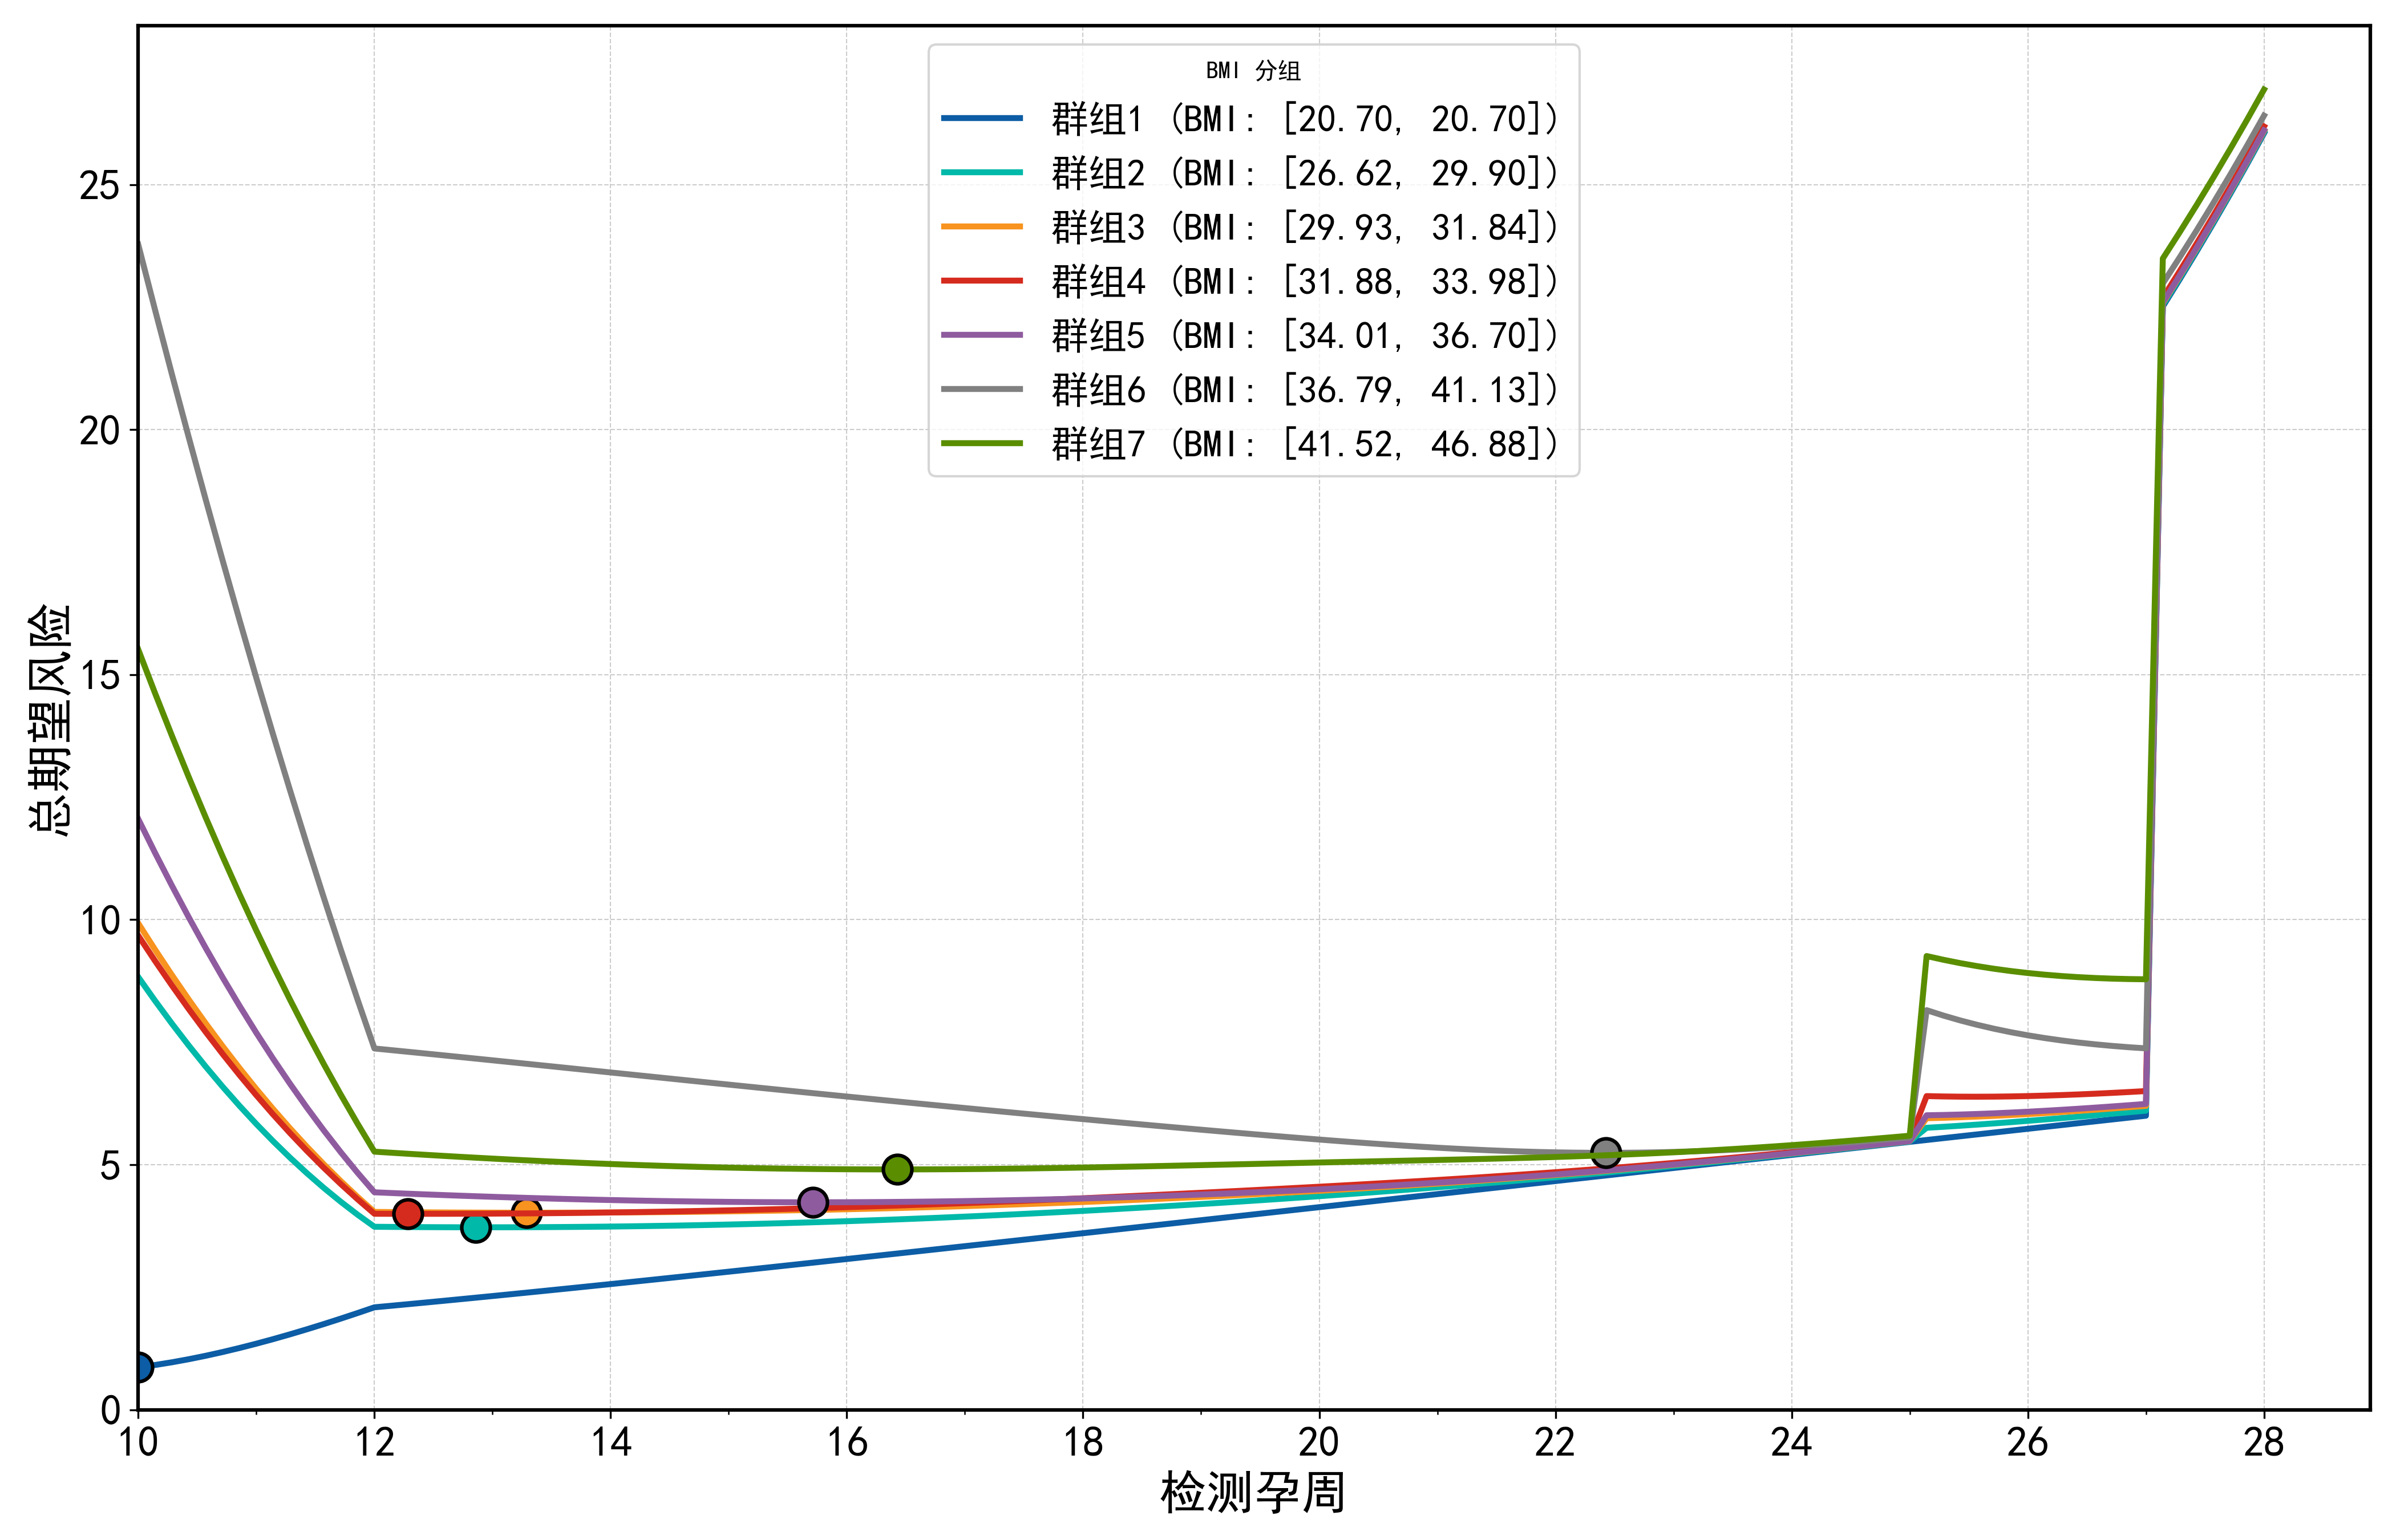
\includegraphics[width=0.9\textwidth]{figs/4问题二/图1_最优分组方案期望风险曲线.png}
\caption{最优分组方案下各群组的期望风险曲线}
\label{fig:q2_risk_curves}
\end{figure}

各群组的最佳检测时点由其总期望风险曲线确定，如\cref{fig:q2_risk_curves}所示。图中每条曲线代表一个BMI群组的总期望风险随检测孕周的变化。所有曲线初期均呈现下降趋势，之后转为上升。曲线的最低点即为该群组风险最小化的最佳检测时点。一个主要趋势是，随着孕妇BMI的升高，风险曲线的最低点向更晚的孕周移动。

\begin{table}[h!]
\centering
\caption{最优分组方案与NIPT时点建议}
\label{tab:final_scheme}
\begin{tabular}{@{}ccccc@{}}
\toprule
群组 & BMI范围 & 孕妇数量 & 最佳时点(周) \\ \midrule
群组1 & [20.70, 20.70] & 4 & 10.0 \\
群组2 & [26.62, 29.90] & 197 & 12.86 \\
群组3 & [29.93, 31.84] & 300 & 13.29 \\
群组4 & [31.88, 33.98] & 260 & 12.29 \\
群组5 & [34.01, 36.70] & 163 & 15.71 \\
群组6 & [36.79, 41.13] & 64 & 22.43 \\
群组7 & [41.52, 46.88] & 10 & 16.43 \\ \bottomrule
\end{tabular}
\end{table}

最终的分组方案与各组别的最佳NIPT时点建议在\cref{tab:final_scheme}中进行了总结。该表明确了每个群组的BMI取值范围与孕妇数量。核心结果体现在最佳时点列，数据显示出BMI与最佳时点的正向关联。BMI最低的群组1，其最佳检测时点为孕10周。BMI较高的群组6，其最佳检测时点则推迟至孕22.43周。此结果为不同BMI的孕妇群体提供了差异化的NIPT检测时间窗口。

\subsection{模型稳定性分析}
为检验模型结论的稳定性，本文从参数敏感性与检测阈值两个维度进行分析。

\begin{figure}[h!]
\centering
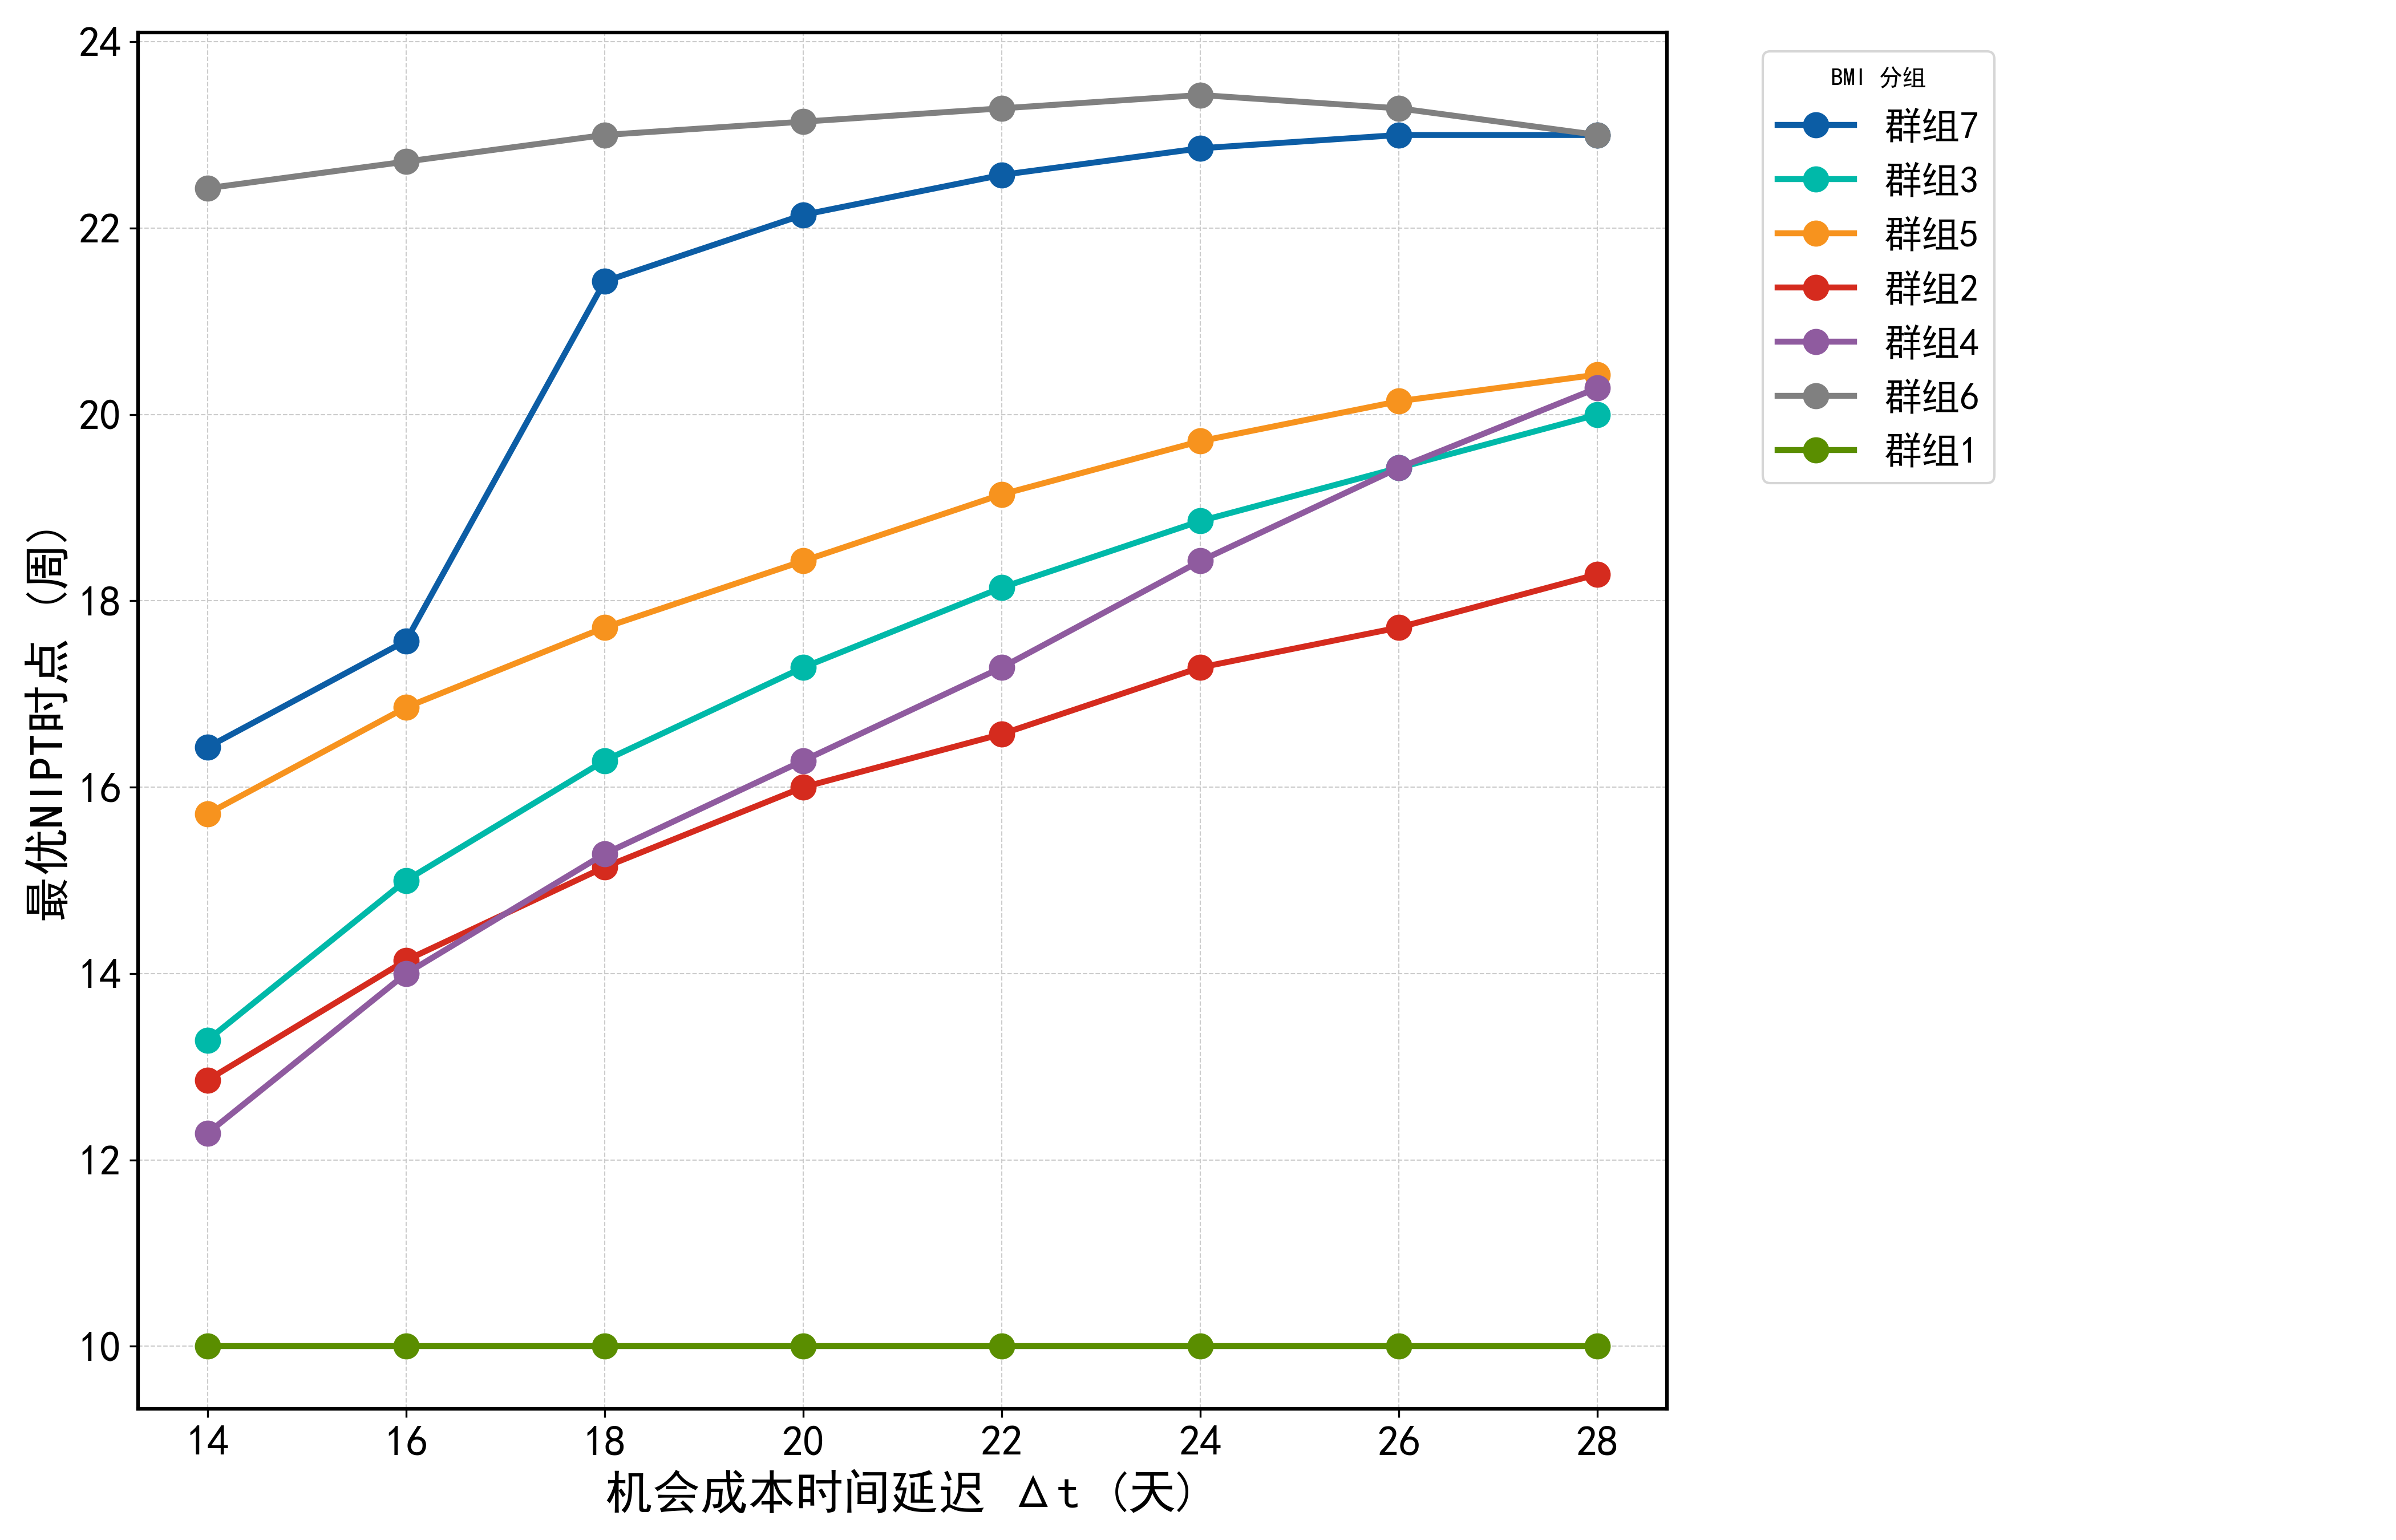
\includegraphics[width=0.8\textwidth]{figs/4问题二/图5_敏感性分析_delta_t.png}
\caption{机会成本时间延迟$\Delta t$的敏感性分析}
\label{fig:q2_sens_delta_t}
\end{figure}

机会成本中的时间延迟参数$\Delta t$对结果的影响如\cref{fig:q2_sens_delta_t}所示。在保持其他参数不变的条件下，调整$\Delta t$在14天至28天的范围内变动。随着时间延迟$\Delta t$的增加，即检测失败的代价变高，多数群组的最佳检测时点均一致性地向更早的孕周移动。此结果符合决策逻辑，当失败后果更严重时，模型会选择一个更早的时间点以降低失败概率。

\begin{figure}[h!]
\centering
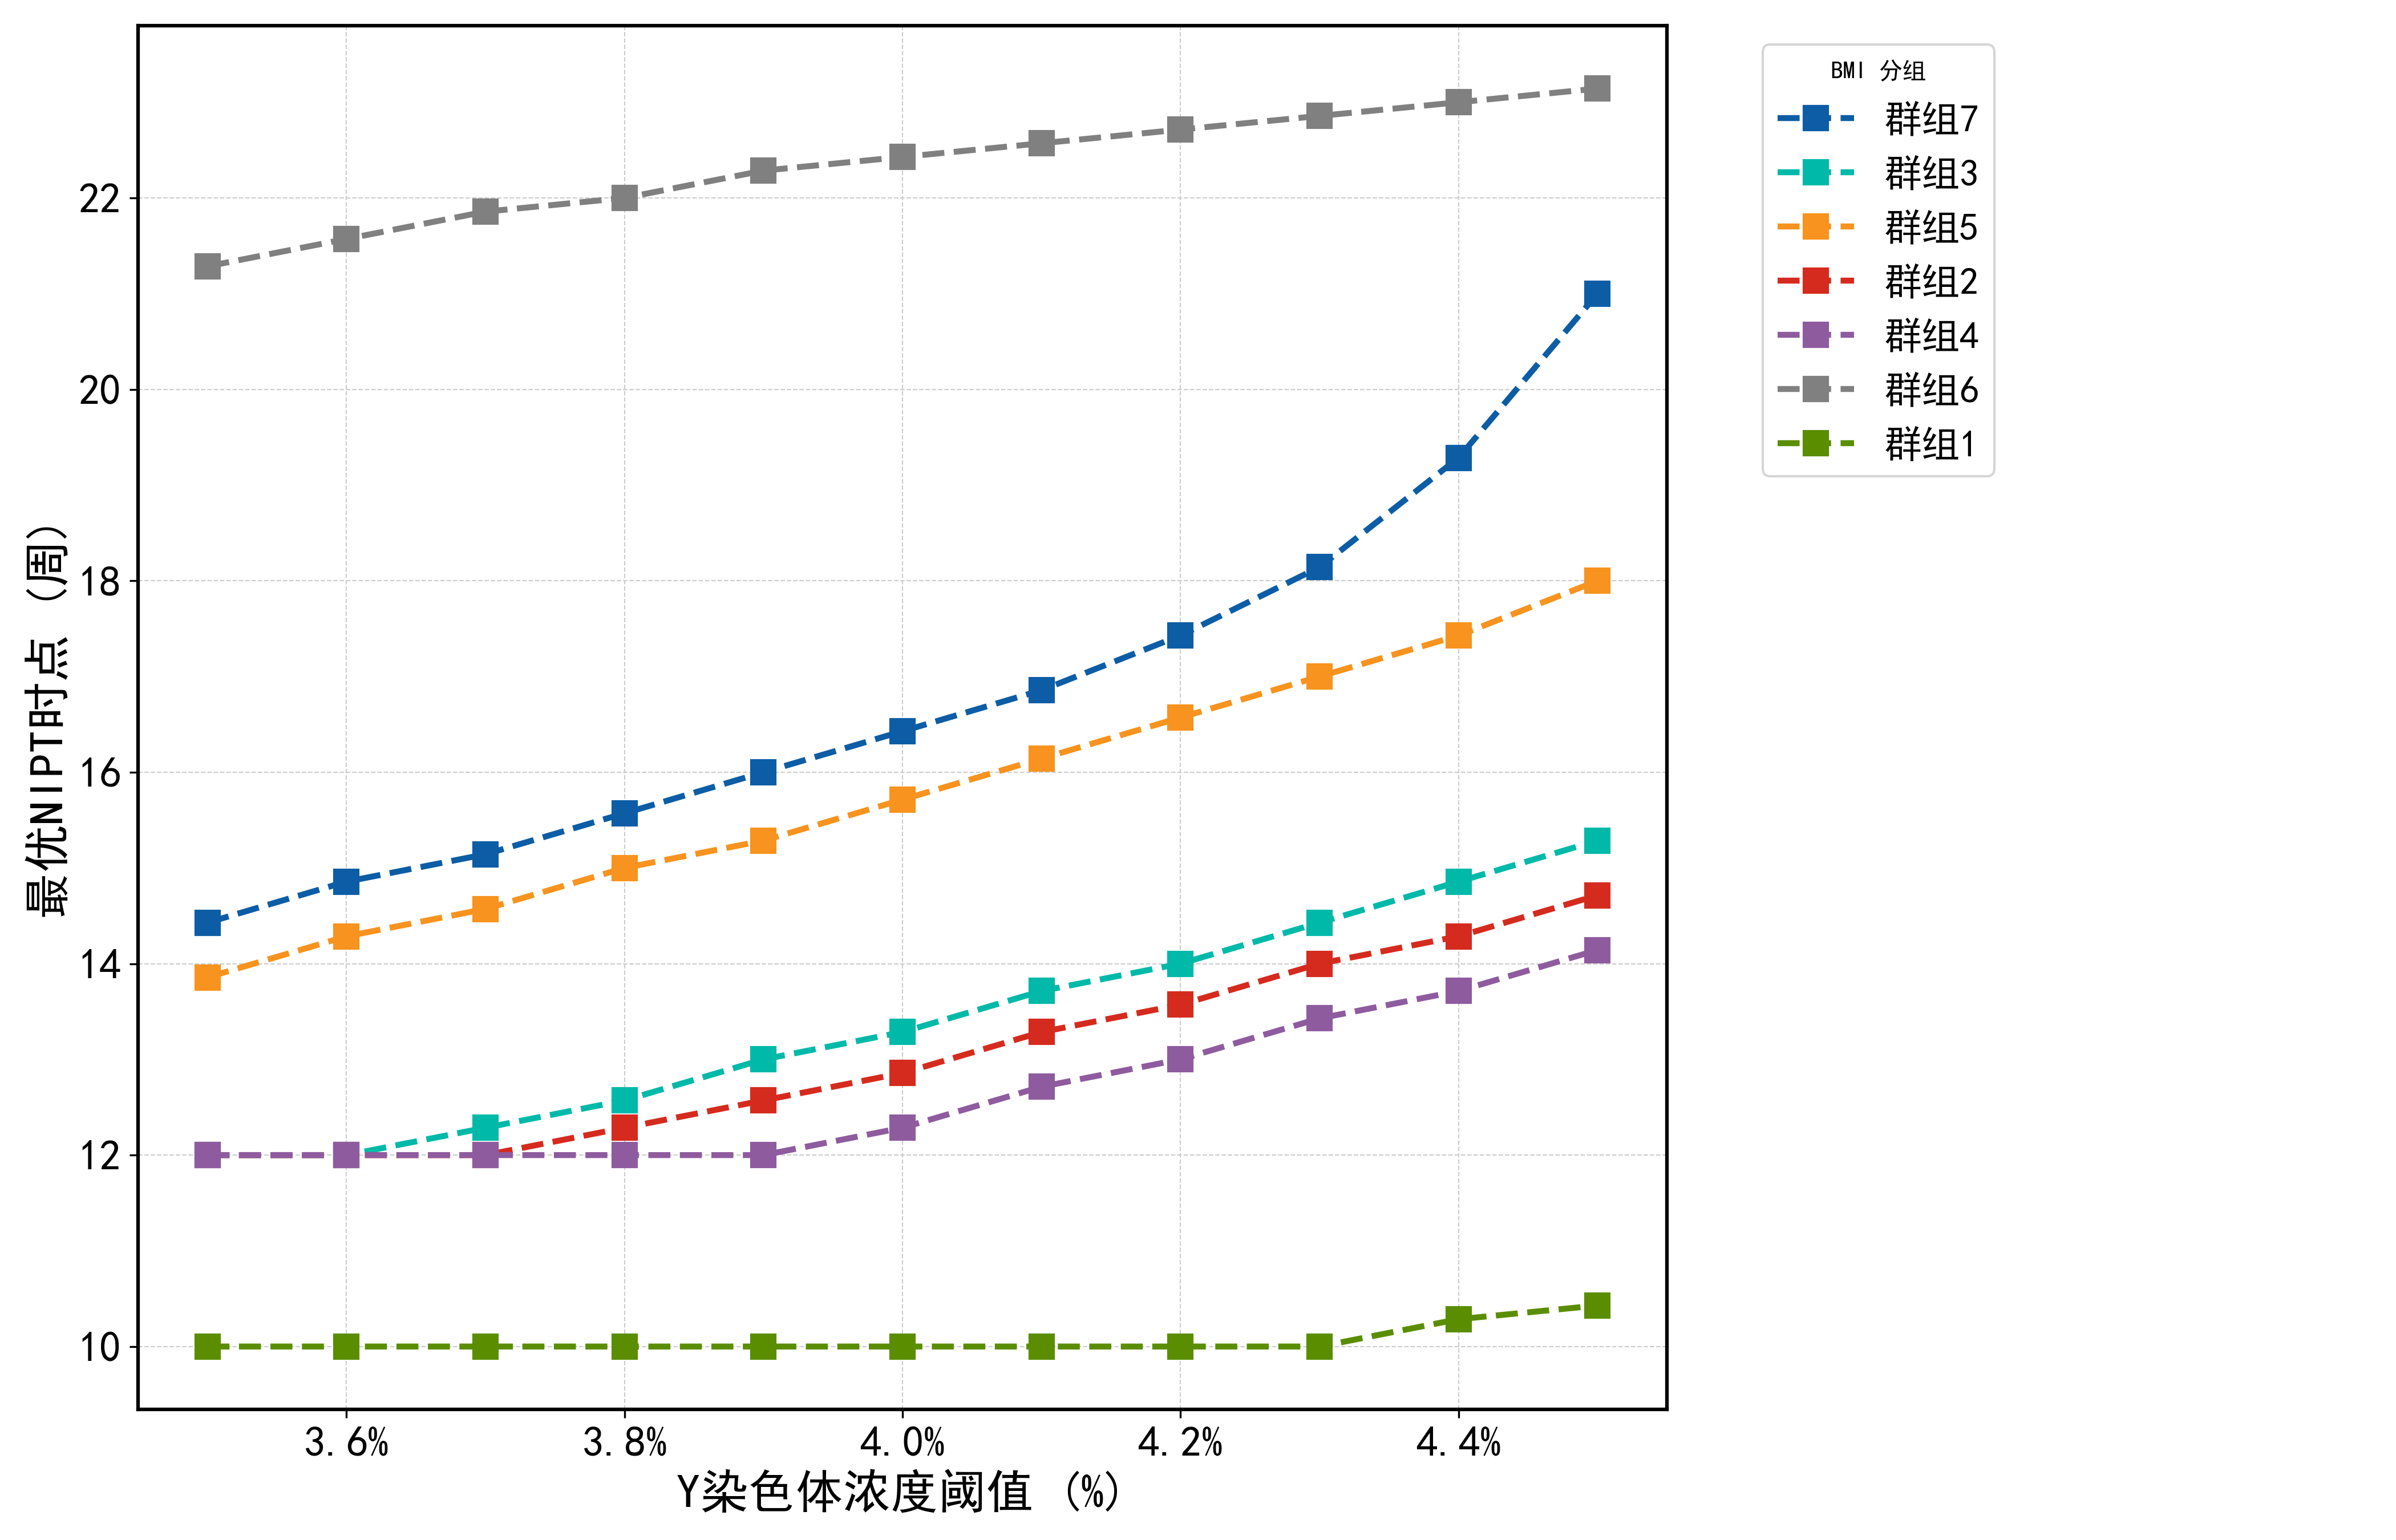
\includegraphics[width=0.8\textwidth]{figs/4问题二/图6_敏感性分析_threshold.png}
\caption{Y染色体浓度阈值对最佳检测时点的影响分析}
\label{fig:q2_sens_threshold}
\end{figure}

为分析NIPT技术标准变化对最优时点策略的影响，本文分析了Y染色体浓度阈值的变动。\cref{fig:q2_sens_threshold}展示了当浓度阈值在3.5\%至4.5\%之间变化时，各组最佳检测时点的变化。随着检测阈值的提高，即成功标准更为严格，各组的最佳检测时点均呈现出系统性的推迟。这表明当检测标准更高时，模型会建议一个更保守的策略，通过适当延长等待时间，来换取Y染色体浓度超过阈值的更高把握。
